\documentclass[professionalfonts,compress,unicode]{beamer}

\usepackage{amsmath,amssymb}
\usepackage{empheq}
\usepackage[utf8]{inputenc}

\usepackage[russian]{babel}

\usepackage{ifthen}

\def\[#1\]{\begin{align*}#1\end{align*}}

\usetheme{Dolgoprudny}
\usecolortheme{FUPM}

\renewcommand{\thefootnote}{\fnsymbol{footnote}}

\graphicspath{{images//}}

\title[УМФ. Уравнение переноса]{Уравнения математической физики\\Уравнение переноса}
\author[Цыбулин И.В.]{Скалько Юрий Иванович\\
\textbf{Цыбулин Иван}}
\date{}
%\vspace{0.3cm}

\begin{document}

{
	\setbeamertemplate{headline}{}
	\setbeamertemplate{footline}{}
	\frame{\titlepage}
}

\newcommand\myframe[3][dup]{
\ifthenelse{\equal{#1}{}}{}{
\ifthenelse{\equal{#1}{dup}}
{\subsection{#2}}{\subsection{#1}}
}\frame{\frametitle{#2}{#3}}}

\section{Уравнения математической физики}

\myframe{Уравнения математической физики}
{
	Основное отличие УМФ от обыкновенных дифференциальных уравнений --- зависимость неизвестной функции
	от многих переменных. В результате, в уравнениях возникают \emph{частные производные}.
	
	Рассмотрим одномерные нестационарные уравнения гиперболического типа:
	\begin{itemize}
		\item Уравнение переноса
		\item Волновое уравнение
		\item Гиперболические системы уравнений
	\end{itemize}
}

\myframe{Гиперболические системы уравнений} 
{
\begin{itemize}
	\item Гиперболические системы уравнений
		\[
		\frac{\partial \mathbf{u}(t,x)}{\partial t} + \mathbf{A}\frac{\partial \mathbf{u}(t,x)}{\partial x} = \mathbf{f}, \quad 
		\mathbf{u} = \begin{pmatrix}u_1\\\vdots\\u_n\end{pmatrix},\,
		\mathbf{A} = \begin{pmatrix}a_{11}&\dots&a_{1n}\\\vdots&\ddots&\vdots\\a_{n1}&\dots&a_{nn}\end{pmatrix}
	\]
	Для гиперболичности требуется, чтобы все собственные числа $\lambda(\mathbf{A})$ были действительными и существовал базис из собственных
	векторов
\end{itemize}
}
\myframe{Уравнение переноса и волновое уравнение} 
{
\begin{itemize}
	\item Уравнение переноса
	\[
	\frac{\partial \rho(t,x)}{\partial t} + c \frac{\partial \rho(t,x)}{\partial x} = f
	\]
	Уравнение описывает перенос некоторой величины (например, плотности $\rho(t,x)$) со скоростью $c$.
	\item Волновое уравнение
	\[
	\frac{\partial^2 E(t,x)}{\partial t^2} - c^2 \frac{\partial^2 E(t,x)}{\partial x^2} = f
	\]
	Уравнение описывает распространение линейных волн (например, электрического поля $E(t,x)$) по среде со скоростью $c$ по всем направлениям.
\end{itemize}
}

\myframe{Волновое уравнение}
{
	Волновое уравнение 
	\[
	\frac{\partial^2 E(t,x)}{\partial t^2} - c^2 \frac{\partial^2 E(t,x)}{\partial x^2} = f
	\]
	легко привести к виду гиперболической системы в переменных $u=\frac{\partial E}{\partial x}, v = \frac{\partial E}{\partial t}$:
	\[
	\frac{\partial v}{\partial t} &- c^2 \frac{\partial u}{\partial x} = f\\
	\frac{\partial u}{\partial t} &- \frac{\partial v}{\partial x} = 0
	\]
	Или в матричном виде
	\[
	\frac{\partial}{\partial t} \begin{pmatrix}u\\v\end{pmatrix} + \begin{pmatrix}
		0 & -c^2\\
		-1 & 0\\
	\end{pmatrix}
	\frac{\partial}{\partial x}\begin{pmatrix}u\\v\end{pmatrix} = \begin{pmatrix}f\\0\end{pmatrix}
	\]
	Легко убедиться, что $\lambda(\mathbf{A}) = \pm c$ и полная система векторов имеется.
}

\section{Численное решение УМФ}
\myframe{Сетка}{
	Для представления численного решения так же, как и в случае ОДУ, необходима \emph{сетка}.
	Отличие от ОДУ в том, что сетка уже не одномерная, а многомерная. Например, для уравнения в переменных $(t,x)$
	необходима двумерная сетка (по времени и пространству)
	
	Соответственно, сеточная функция будет иметь несколько индексов. Условимся $u^n_m$ обозначать
	значение сеточной функции $u$ на временном слое $n$ в пространственной точке $m$
	\begin{figure}%
	\includegraphics[width=0.6\columnwidth]{grid.pdf}%
	\end{figure}
}

\myframe{Шаблон}{
	Пусть для вычисления $u^{n+1}_m$ требуются значения функции $u$ в нескольких сеточных узлах.
	Тогда эти узлы вместе с узлом $(n+1,m)$ образуют \emph{шаблон разностной схемы}.
	
	Шаблон часто изображают графически, например для схемы <<явный левый уголок>> шаблон выглядит так:
	\begin{figure}%
	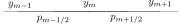
\includegraphics[width=0.3\columnwidth]{stencil.pdf}%
	\end{figure}
	
	Некоторые выводы о разностной схеме можно сделать изучив только ее шаблон
}

\myframe{Область зависимости решения разностной задачи}
{
	Выберем узел сетки $(n+1,m)$. Отметим все узлы сетки, которые нужны для вычисления $u^{n+1}_{m}$. 
	Мы получим шаблон разностной схемы. К каждому новому узлу снова применим ту же процедуру.
	В результате получится некоторый конус --- \emph{область зависимости решения разностной задачи}
	\begin{figure}%
	\includegraphics[width=0.6\columnwidth]{grid_dep.pdf}%
	\end{figure}	
	Все узлы, которые не попали в этот конус не могут влиять на решение в узле $(n+1,m)$
}

\myframe{Область зависимости решения дифф. задачи}
{
	Все уравнения гиперболического типа имеют характеристики. 
	Если из точки $t_{n+1}, x_m$ выпустить все характеристики, то область от самой левой
	до самой правой характеристики будет \emph{областью зависимости решения дифференциальной задачи}
	
	Например, уравнение переноса 
	\[
	\frac{\partial u}{\partial t} + c \frac{\partial u}{\partial x} = 0
	\]
	имеет только одну характеристику $x - ct = \operatorname{const}$. Область зависимости в этом случае --- луч
	$x - ct = x_m - ct_{n+1}, t < t_{n+1}$
	\begin{figure}%
	\includegraphics[width=0.5\columnwidth]{grid_dep2.pdf}%
	\end{figure}		
}

\myframe{Условие Куранта-Фридрихса-Леви}
{
	Если область зависимости решения дифференциальной задачи не содержится целиком в области 
	зависимости решения разностной задачи, то решение разностной задачи не может
	сходиться к решению	дифференциальной.
	
	Действительно, изменим решение в той части области, которая лежит в области зависимости дифференциальной задачи,
	но которая не лежит в области зависимости разностной задачи. Решение разностной задачи при этом не изменится,
	а дифференциальной - изменится. Такое поведение не зависит от выбора мелкости сетки (при условии сохранения пропорций между $\tau$ и $h$),
	следовательно сходимость не возможна.
}

\myframe{Аппроксимация}
{
	Изучение аппроксимации, как и для ОДУ, производится при помощи подстановки в разностную
	задачу проекции точного решения $y(t,x)$	
	\[u^n_m = [y]^n_m\]
	При этом в разностном уравнении появится невязка $\delta^n_m$. Невязка вычисляется путем подстановки
	вместо $[y]^{n'}_{m'}$ разложения в ряд Тейлора относительно некоторой точки $(t_n,x_m)$.
	
	Поскольку разложение в ряд Тейлора производится уже функции многих переменных, желательно 
	выписывать разложение в ряд Тейлора относительно точки на пересечении линий шаблона, 
	при этом из ряда Тейлора исчезают смешанные производные.
}

\myframe{Некоторые схемы для уравнения переноса}
{
	\begin{itemize}
		\item Явный левый уголок
		\[
		\frac{u^{n+1}_m-u^n_m}{\tau} + c \frac{u^{n}_m-u^n_{m-1}}{h} = f_m^n
		\]
		\item Явный правый уголок
		\[
		\frac{u^{n+1}_m-u^n_m}{\tau} + c \frac{u^{n}_{m+1}-u^n_m}{h} = f_m^n
		\]
		\item Схема с центральной разностью
		\[
		\frac{u^{n+1}_m-u^n_m}{\tau} + c \frac{u^{n}_{m+1}-u^n_{m-1}}{2h} = f_m^n
		\]
		\item Схема Лакса
		\[
		\frac{u^{n+1}_m-\frac{1}{2}\left(u^n_{m-1}+u^n_{m+1}\right)}{\tau} + c \frac{u^{n}_{m+1}-u^n_{m-1}}{2h} = f_m^n
		\]		
	\end{itemize}
}

\myframe{Изучение аппроксимации}
{
	Подставим разложения
	\[
	[y]^{n+1}_m &= [y]^n_m + \tau [y_t]_m^n + \frac{\tau^2}{2} [y_{tt}]_m^n + O(\tau^3)\\
	[y]^n_{m \pm 1} &= [y]^n_m \pm h[y_x]_m^n + \frac{h^2}{2} [y_{xx}]_m^n \pm \frac{h^3}{6} [y_{xxx}]_m^n + \frac{h^4}{24} [y_{xxxx}]_m^n + O(h^5)
	\]
	в схему явный левый уголок
	\[
	&[y_t]_m^n + \frac{\tau}{2} [y_{tt}]_m^n + O(\tau^2) + c\left([y_x]_m^n - \frac{h}{2} [y_{xx}]_m^n + O(h^2)\right) = f^n_m + \delta\\
	&([y_t]_m^n+c[y_x]_m^n-f_m^n) + \frac{\tau}{2} [y_{tt}]_m^n + O(\tau^2) - c\left(\frac{h}{2} [y_{xx}]_m^n + O(h^2)\right) = \delta\\
	&\delta = \frac{\tau}{2}[y_{tt}]_m^n - \frac{ch}{2}[y_{xx}]_m^n + O(\tau^2+h^2) = O(\tau+h)
	\]
	Схема имеет первый порядок аппроксимации по времени и пространству
}

\myframe[]{Изучение аппроксимации}
{
	Подставим разложения
	\[
	[y]^{n+1}_m &= [y]^n_m + \tau [y_t]_m^n + \frac{\tau^2}{2} [y_{tt}]_m^n + O(\tau^3)\\
	[y]^n_{m \pm 1} &= [y]^n_m \pm h[y_x]_m^n + \frac{h^2}{2} [y_{xx}]_m^n \pm \frac{h^3}{6} [y_{xxx}]_m^n + \frac{h^4}{24} [y_{xxxx}]_m^n + O(h^5)
	\]
	В схему с центральной разностью
	\[
	&[y_t]_m^n + \frac{\tau}{2} [y_{tt}]_m^n + O(\tau^2) + c\left([y_x]_m^n + \frac{h^2}{6} [y_{xxx}]_m^n + O(h^4)\right) = f^n_m + \delta\\
	&([y_t]_m^n+c[y_x]_m^n-f_m^n) + \frac{\tau}{2} [y_{tt}]_m^n + O(\tau^2) + c\left(\frac{h^2}{6} [y_{xxx}]_m^n + O(h^4)\right) = \delta\\
	&\delta = \frac{\tau}{2}[y_{tt}]_m^n + \frac{ch^2}{6}[y_{xxx}]_m^n + O(\tau^2+h^4) = O(\tau+h^2)
	\]
	Схема имеет первый порядок аппроксимации по времени и второй по пространству
}

\myframe[]{Изучение аппроксимации}
{
	Подставим разложения
	\[
	[y]^{n+1}_m &= [y]^n_m + \tau [y_t]_m^n + \frac{\tau^2}{2} [y_{tt}]_m^n + O(\tau^3)\\
	[y]^n_{m} &= [y]^n_m \pm h[y_x]_m^n + \frac{h^2}{2} [y_{xx}]_m^n \pm \frac{h^3}{6} [y_{xxx}]_m^n + \frac{h^4}{24} [y_{xxxx}]_m^n + O(h^5)
	\]
	В схему Лакса
	\[
	&[y_t]_m^n + \frac{\tau}{2} [y_{tt}]_m^n + O(\tau^2) + \frac{h^2}{2\tau}[y_{xx}]_m^n + O\left(\frac{h^4}{\tau}\right) + \\
	&+c\left([y_x]_m^n + \frac{h^2}{6} [y_{xxx}]_m^n + O(h^4)\right) = f^n_m + \delta\\
	&([y_t]_m^n+c[y_x]_m^n-f_m^n) + \frac{\tau}{2} [y_{tt}]_m^n + O(\tau^2) + \frac{h^2}{2\tau}[y_{xx}]_m^n + O\left(\frac{h^4}{\tau}\right) +\\
	&+c\left(\frac{h^2}{6} [y_{xxx}]_m^n + O(h^4)\right) = \delta\\
	\]
}

\myframe[]{Изучение аппроксимации}
{
	Для схемы Лакса
	\[
	\delta &= \frac{\tau}{2} [y_{tt}]_m^n + \frac{h^2}{2\tau}[y_{xx}]_m^n + c\frac{h^2}{6} [y_{xxx}]_m^n +  O\left(\tau^2 + \frac{h^4}{\tau} + h^4\right) \\
	\delta &= O\left(\tau + \frac{h^2}{\tau} + h^2\right) = O\left(\tau + \frac{h^2}{\tau}\right)
	\]
	
	Аппроксимация схемы зависит от соотношения между $\tau$ и $h$. Например, если $\tau = O(h)$, то схема имеет первый порядок по пространству и времени,
	а если $\tau = O(h^2)$, то ошибка аппроксимации $O(1)$, то есть аппроксимации нет. (Есть аппроксимация \emph{другого} уравнения)
}

\myframe{Устойчивость}
{
	Исследуем левый уголок на устойчивость. Из условия КФЛ можно сразу сказать, что при $\frac{c\tau}{h} > 1$ или $\frac{c\tau}{h} < 0$ устойчивости не будет,
	так как нет сходимости, а аппроксимация есть. (Иначе по теореме Рябенького аппроксимация + устойчивость = сходимость).
	
	Чтобы производить расчеты по схеме <<левый уголок>> необходимы еще данные на левой границе и на начальном слое по времени
	\[
	&u^0_m = \varphi_m\\
	&u^n_0 = \psi^n
	\]
	
}

\myframe[]{Устойчивость}
{
	Перепишем схему в виде
	\[
	&u^{n+1}_m = u^n_m + \frac{c\tau}{h}\left(u^n_{m-1}-u^n_m\right)+\tau f_m^n, \quad m=\overline{1,M}\\
	&u^{n+1}_m = \left[1-\frac{c\tau}{h}\right] u^n_m + \frac{c\tau}{h}u^n_{m-1}+\tau f_m^n, \quad m=\overline{1,M}\\
	&|u^{n+1}_m| \leq \left|1-\frac{c\tau}{h}\right||u^n_m| + \left|\frac{c\tau}{h}\right||u^n_{m-1}|+\tau |f_m^n|, \quad m=\overline{1,M}
	\]

	Вводя нормы
	\[
	\|u^n\| = \max_{m=\overline{0,M}} |u^n_m|, \quad
	\|u\| = \max_{n=\overline{0,N}} \|u^n\|,
	\]
	можно записать
	\[
	\|u^{n+1}\| \leq \max\left\{|u_0^{n+1}|,
	\left(1-\frac{c\tau}{h}\right)\max_{m>0}|u^n_m|+
	\frac{c\tau}{h}\max_{m>0}|u^n_{m-1}|+ \tau \|f^n\|
	\right\}
	\]
}

\myframe[]{Устойчивость}
{
	\[
	\|u^{n+1}\| \leq \max\left\{|u_0^{n+1}|,
	\left(1-\frac{c\tau}{h}\right)\max_{m>0}|u^n_m|+
	\frac{c\tau}{h}\max_{m>0}|u^n_{m-1}|+ \tau \|f^n\| \right\}
	\]
	Оценив $\max\limits_{m>0}|u^n_{m-1}| \leq \|u^n\|, \max\limits_{m>0}|u^n_{m}| \leq \|u^n\|$
	\[
	&\|u^{n+1}\| \leq \max \{|\psi^{n+1}|, \|u^n\|+\tau \|f^n\|\} \leq \max \{|\psi^{n+1}|, \|u^n\|\}+\tau \|f\|\leq\\
	&\leq \max \{|\psi^{n+1}|, |\psi^n|, \|u^{n-1}\|\}+2\tau \|f\| \leq \dots \leq \max \{\|\psi\|, \|\varphi\|\}+T \|f\|
	\]
	Получаем
	\[
	\|u\| \leq \|\psi\|+\|\varphi\|+T\|f\|
	\]
	Это доказывает устойчивость задачи по правой части, начальным и граничным условиям.
}

\myframe{Монотонные схемы}
{
	Оказывается, если схему можно представить в виде
	\[
	u^{n+1}_m = \sum_{\mu} \alpha_\mu u^n_{m+\mu}
	\]
	причем все $\alpha_\mu > 0$, то доказательство устойчивости полностью аналогично доказательству устойчивости для явного левого уголка.
	Такие схемы называются монотонными. К сожалению, монотонных схем выше первого порядка аппроксимации не бывает. Запишем схему Лакса в такой форме
	\[
	u^{n+1}_m = \left(\frac{1}{2}+\frac{c\tau}{2h}\right) u^n_{m-1} + \left(\frac{1}{2}-\frac{c\tau}{2h}\right) u^n_{m+1}
	\]
	Схема устойчива при $\left|\frac{c\tau}{h}\right| \leq 1$, а при нарушении этого условия неустойчива по условию КФЛ.
}

\myframe{Спектральный признак}
{
	Доказательство устойчивости по определению бывает довольно сложной задачей. 
	В этой случае можно воспользоваться спектральным признаком устойчивости. Хотя он и не является
	строгим критерием, зачастую он дает правильный результат.
	
	Спектральным признаком можно исследовать только \emph{задачу Коши}, то есть задачу без граничных условий, только 
	с начальными. Эта задача исследуется на устойчивость только по начальным данным, возмущение правой части всегда полагается равным $0$.
	Из всех возможных возмущений начальных условий изучаются только возмущения вида $u^0_m = e^{i\alpha m}$. Поскольку 
	любую функцию можно представить в виде интеграла Фурье, такое сужение допустимо.
}

\myframe[Спектральный признак для схемы O(т+h2)]{Спектральный признак для схемы $O(\tau+h^2)$}
{
	Рассмотрим задачу 
	\[
	&\frac{u_m^{n+1}-u^n_m}{\tau} + c\frac{u^n_{m+1}-u^n_{m-1}}{2h} = 0\\
	&u^0_m = e^{i \alpha m}
	\]
	Найдем $u^1_m$
	\[
	u^1_m = u^0_m + \frac{c\tau}{h}\frac{u^0_{m+1}-u^0_{m-1}}{2} = u^0_m \left(1 + i \frac{c\tau}{h} \sin \alpha\right)
	\]
	Аналогично,
	\[
	u^n_m = \left(1 + i \frac{c\tau}{h} \sin \alpha\right)^n e^{i\alpha m}
	\]
	Решение такой задачи всегда можно искать в виде $u^n_m = \lambda^n e^{i \alpha m}$.
}

\myframe[]{Спектральный признак для схемы $O(\tau+h^2)$} 
{
	Найдем норму $u_m^n$
	\[
	\|u\| = \max_m \max_{n=\overline{0,N}} |\lambda^n e^{i \alpha m}| = \max_{n=\overline{0,N}} |\lambda^n| = \max(1, |\lambda|^{N})
	\]
	\begin{itemize}
		\item Если $|\lambda| \leq 1$, то решение ограничено константой ($C = 1$), умноженной на возмущение начальных условий, то есть задача устойчива.
		\item Если $|\lambda| = 1 + D\tau$, то решение ограничено константой ($C = (1 + D\tau)^{T/\tau} \leq e^{DT}$), то есть задача тоже устойчива. 
	Однако, чем больше константа $D$, тем сильнее зависимость возмущения решения от возмущения начальных условий, тем менее устойчива задача.
		\item Если $\frac{|\lambda|-1}{\tau} \rightarrow \infty$, то задача неустойчива.
	\end{itemize}
	Довольно часто задача полагается неустойчивой при $|\lambda| > 1$, хотя это не совсем строго.
}

\myframe[]{Спектральный признак для схемы $O(\tau+h^2)$} 
{
	Рассмотрим схему с 
	\[
	\lambda = 1 + i \frac{c\tau}{h} \sin \alpha\\
	|\lambda| = \sqrt{1 + \frac{c^2\tau^2}{h^2}\sin^2 \alpha} > 1
	\]
	При $\tau = O(h),\quad \frac{|\lambda| - 1}{\tau} = O\left(\frac{1}{\tau}\right) \rightarrow \infty$. Схема неустойчива.
	
	При $\tau = O(h^2), \quad |\lambda| = \sqrt{1 + c\tau\sin^2\alpha} \approx 1 + \frac{c\sin^2\alpha}{2}\tau \leq 1 + \frac{c}{2}\tau$.
	Схема устойчива с константой $C = e^{\frac{cT}{2}}$
}

%%%%%%%%%%%%%%%%%%%%%%%%%%%%%%%%%%%%%%%%%%%%%%%
%%%%%%%%%%%%%%%%%%%%%%%%%%%%%%%%%%%%%%%%%%%%%%%
%%%%%%%%%                            %%%%%%%%%%
%%%%%%%%%%%%%%%%%%%%%%%%%%%%%%%%%%%%%%%%%%%%%%%
%%%%%%%%%%%%%%%%%%%%%%%%%%%%%%%%%%%%%%%%%%%%%%%
{
\setbeamertemplate{headline}[default] 
\frame{
	\begin{center}
	{\Huge Спасибо за внимание!}
	\end{center}
	\bigskip
	\begin{center}
	{\color{blue}{tsybulin@crec.mipt.ru}}
	\end{center}
	}
}

\end{document}
